\documentclass[a4paper,11pt,titlepage]{article}
\usepackage{graphicx}
\author{Abrie Greeff\\B.Sc Hons (Computer Science)\\Department of Computer Science\\University of Stellenbosch}
\title{Virtual Clay Modeling using Cellular Automata}
\begin{document}
\maketitle
\tableofcontents
\section{Introduction}
3D modeling has become a very important part in the creation of visual tools. 3D models are used in a wide field of computer applications. These range from architectural designs to computer generated movie scenes. A number of techniques exist to create these models. The technique we will be examining is called free-form modeling.\\
Free-form modeling is a technique used to model objects by building them from an initial object and then modifying this object to obtain the preferred result. When an entity wants a specific model this method enables them to easily create this model because of the similarities between free-form modeling and modeling objects in the physical world. The main problem with this method is if the application used for the modeling doesn't accurately represent the laws of physics as experienced in the real world. This may cause the object to behave incorrectly when a model is formed.\\
Research has been carried out on many different methods using physical laws to obtain real-time free-form modeling. Unfortunately because of the complex shapes the computational time needed to deform the objects wasn't suitable for real-time interaction. To address this problem easier solutions that have less computation time needed to be found. One such approach is the division of the object into small voxels (or pixels in 2D). Every voxel can have its contents changed to represent a part of the object. A method that uses this idea and combines this with a cellular automata (CA) was proposed in [1].\\
This method views the object as one big mass of clay. The deformation of the object to obtain the model is then simulated as virtual clay modeling. This is the same concept as clay modeling in the physical world. The deformation of the clay is based upon a set of distribution rules applied to the CA. Every voxel is assigned one finite state automata that is part of the CA. Every state of the CA performs state transitions based upon the state of its neighbours.\\
This paper examines this method of free-form modeling. Only the two-dimensional case will be studied and implemented.
\section {Virtual Clay Modeling}
The clay is seen as a block of cells. Initially every cell will represent an amount of the clay that has been distributed equally between all the cells in the block. These values in every cell will be the fraction of the mass of the clay that this cell contains. Because the cell has mass and constant volume the cell also has the property that it has density. The density of a cell is used in the transition function of every state. All states in the CA has the same density threshold and when this threshold is broken a state's mass needs to be repartitioned to confer with physical laws. This causes the clay to deform and hopefully have the same deformation as real clay would in the physical world.\\
When a cell needs to be repartitioned it will distribute a certain amount of clay between its neighbours who are under the threshold. This amount will be specified by the repartition rule. A cell decides whom it wants to distribute its excess clay to by looking at its Margolus neighbourhood. When it knows what neighbours are under threshold the repartition rule is used to decide the distribution. The Margolus neighbourhood and the repartition rule are discussed in the sections that follow.

To deform the clay a plate of an arbitrary size is pushed against the clay from a chosen angle. When this plate pushes against the clay all the cells it touches distribute their contents to the cells adjacent to them.
This causes the clay to have parts where the density is greater than the threshold. This causes the CA to execute its transition functions which in turn causes the clay to deform.
\subsection {Margolus Neighbourhood}
In a Margolus neighbourhood the 4 nearest neighbour cells make up one block. This block includes the cell currently being looked at. The boundaries of the cell that is being looked at is changed every iteration. There are two types of steps, the even step and the odd step. The Margolus neighbourhood for these two steps are shown in fig 1.

\begin{figure}[htbp]
   \centering
   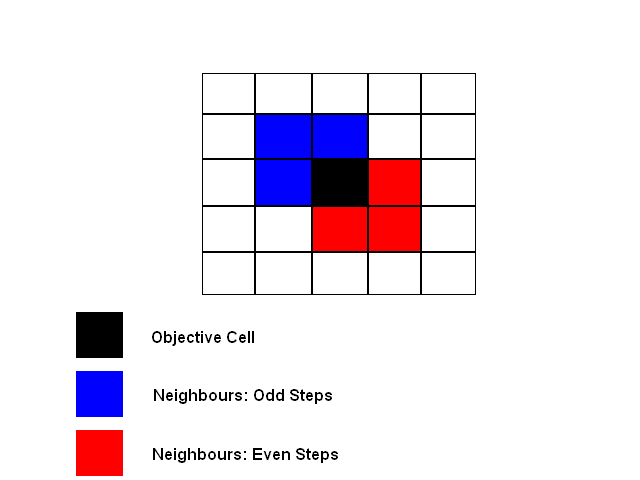
\includegraphics[width=10cm]{bure.png}
   \caption{Margolus neighbourhood}
   \label{Figure:figex}
\end{figure}

Each cell in the neighbourhood that is over the threshold is then repartitioned according to the repartition rule. The transitions that is applied on the cells in the neighbourhood are shown in fig. 2 for the even step and in fig. 3 for the odd steps.
There are four possible cases for each step that can occur depending if the neighbours are over the threshold.
\begin{figure}[htbp]
   \centering
   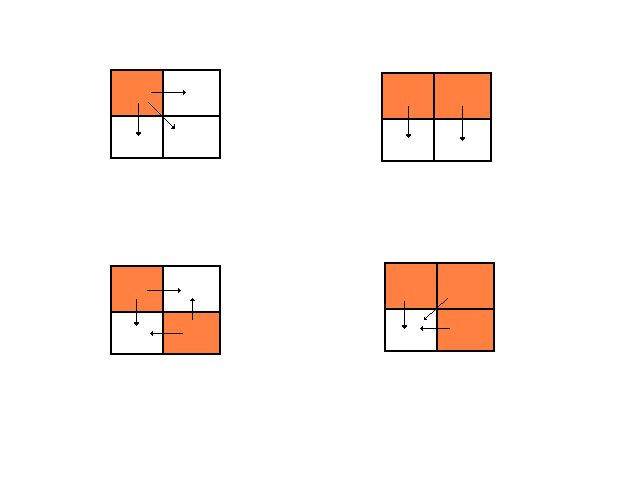
\includegraphics[width=10cm]{even.png}
   \caption{Repartitioning: Even step}
   \label{Figure:figex}
\end{figure}
\begin{figure}[htbp]
   \centering
   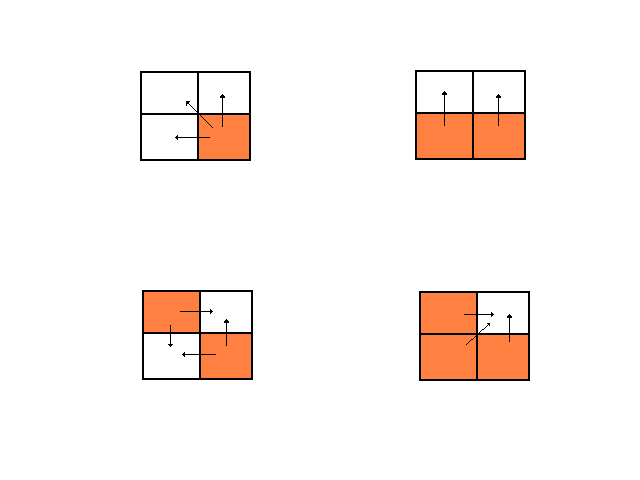
\includegraphics[width=10cm]{odd.png}
   \caption{Repartitioning: Odd step}
   \label{Figure:figex}
\end{figure}
\subsection {Repartition Rule}
The repartition rule is defined as follows,\\*
\\*
For each block\\
For each cell \emph{k} over threshold\\
	$ dm_k \gets m_k * \alpha $\\
	$ m_k \gets m_k - dm_k$\\*
For each cell \emph{j} under threshold\\
	$m_j \gets m_j + ( dm_1 + dm_2 +... + dm_r ) / n$\\*
\\
where $m_k$ and $m_j$ is the mass of cell \emph{k}, $\alpha$ is a rate constant for distribution $( 0 < \alpha < 1 )$, $dm_k$ the portion of the mass that is being redistributed, \emph{r} the number of cells over threshold and \emph{n} the amount of cells under threshold.
\newpage
\section{Implementation}
The virtual clay system CA was implemented in Java. The structure used to store the CA was a $n \times n$ array with every index consisting of a floating point number.
This floating point number was used to represent the amount of mass present in every cell of the CA. This structure was chosen because the time it takes to index any given cell is \emph{O(1)} and it isn't known beforehand if all the cells will be used because of the dynamic growth of the system when it's being sculpted.
Index time is the most important factor in this system because the objective of the system is to be as fast as possible. This fast index time allows the system almost real time computation and satisfies the most important objective of the application.

The application runs in a full screen graphical mode. This enables the program to execute faster because the graphics card can concentrate on this application. Drawing of the system on the screen happens after every odd or even step to furthermore improve efficiency. This probably could have been improved further if the drawing of the system was a separate thread from the main program.
This would have enabled separation between the two main functions of the program. Therefore enabling each one to concentrate on their own goal.

The program was first divided in to two main parts. The first part was obtaining the data needed to initialize the clay before it is deformed. The second part was the actual deformation of the clay. The movement of the plate was limited to one direction because this application only serves as an example of virtual clay modeling. It was chosen that the plate will only move vertically down to compare the results with those obtained in [1] and [2].

\subsection{Initial configuration}
Before the deformation phase could be started three things are needed from the user of the application. Firstly the user must inform the application how big the CA must be. This value constructs a grid on the screen. As this value increases the size of each cell is decreased thus creating a finer grid that allows better results in the deformation phase. The problem of a very fine grid is that the time for each iteration is also much longer because more cells needs to be visited each time.
To receive this information from the user an input box is presented at the start of the program. This increases the interactivity of the program and eliminates the need for unnecessary setup of text files before the program is executed.

The second thing that is needed from the user is where the clay is situated and what form it is. This is done by dragging the mouse on the grid on the screen and drawing the block of clay. 
It was made possible to redraw the clay because it may be possible that the user didn't draw the clay as he/she may have wanted it to be.

The last thing that the application needs from the user is to know where the plate must be put. This is done in exactly the same way as the drawing of the clay. The only difference is the user needs to hold down the \emph{Space bar} key while drawing the plate. 
The drawing of both of these objects was made independent from each other. This enables full control over how the system should look before deformation of the clay happens.
Once the user is happy with his/her choices the \emph{Enter} key can be pressed and the program begins the deformation phase.
\subsection{Deformation phase}
The deformation phase consist of two main functions. These are the running of the CA and the drawing of the clay on the screen.
\subsubsection{Drawing the clay}
The drawing of the clay is a very important part of the whole application. This is the only way the user can see if the deformation of the clay is happening as it would be expected to happen in the physical world. The clay is drawn as varying intensities of the color green.
These intensities each represent the density of the clay in that particular cell. The brighter the green is displayed on the screen the higher the density of the cell is. 
The plate is shown as a red block on the screen.
This is shown in fig. 4.
\begin{figure}[htbp]
   \centering
   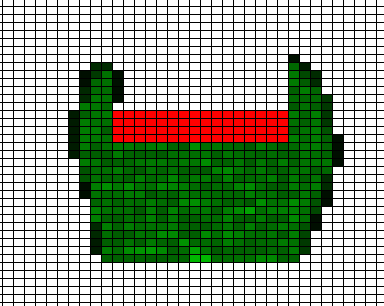
\includegraphics[width=8cm]{example1.png}
   \caption{Example of a possible clay deformation}
   \label{Figure:figex}
\end{figure}

\subsubsection{The cellular automata}
The CA was executed in two phases. The first phase was running all the even steps on the whole CA. For every cell the distribution function was called on the Margolus neighbourhood as explained in Section 2. When the even steps were done the second phase was executed. This consisted of running the odd steps on the CA.
When this finished the whole CA was checked to see if any cells where still over the threshold. If this was the case the first phase was repeated again followed by the second phase.

When there wasn't any cells over the threshold it meant we were able to move the plate down one row. If this caused any cells to be over the threshold the whole process was repeated again from the first phase. This repeated until the system reached a stable state where all the cells were under the threshold and the plate had stopped moving.

\section{Testing}
The main idea behind the tests that were performed on the application was to see if the clay behaved correctly under deformation. There were two main tests that were executed on the program. 
The first test consisted of a block of clay being pushed down by a plate that is wider than the block of clay. The second test was a block of clay where the plate was narrower than the width of the block of clay.

The tests quickly showed that the algorithm described in [1] doesn't correctly explain how it must be implemented.
The clay spread at its base making it look like a thick fluid flowing away from it. This was definitely incorrect because the desired form of the clay should have been in the form of a mushroom, like a pillar at the base with a big head at the top that is expanding. The error was because [1] and [2] doesn't clearly state that after a objective cell has been inspected the next objective cell shouldn't have that cell in its neighbourhood.
When this was corrected the expected mushroom effect started to appear when the program executed.

When tests was performed again it showed that the algorithm doesn't accurately represent the physical laws of clay deformation. The deformation was however satisfactory for a small system.
\newpage
\section{Conclusion}
Overall the free-form deformation of clay was very satisfactory. It may be possible to further improve these results by using the partition rules as mentioned in [2]. It was interesting to notice how the system started to slow down when the plate neared the bottom of the clay. Overall system performance wasn't real time and could have been improved with better use of threads. 
This is the biggest problem because the goal of the system is to be real time. However faster computers may eliminate this problem in the future.
\section{References}
\begin{enumerate}
\item H. Arata, Y. Takai, N. K. Takai, and T. Yamamoto.
\emph{Free-form shape modeling by 3D cellular automata.} International Conference on Shape Modeling and Applications, pages 242-247, 1999
\item S. Druon, A. Crosnier, and L. Brigandat.
\emph{Efficient Cellular Automata for 2D / 3D Free-form Modeling.} Journal of WSCG 2003, vol.11, No.1
\end{enumerate}
\end{document}
